\documentclass[11pt,french]{report}
% % Numéro de page gauche et droite
% \documentclass[11pt,french,twoside]{report}
% usepackage{titleps} = usepackage[pagestyles]{titlesec}
% \renewpagestyle{plain}{%
% \sethead{}{}{}
% \setfoot[\thepage][][]{}{}{\thepage}
% }%
% \pagestyle{plain}
\usepackage{float}
\usepackage[utf8]{inputenc}
\usepackage[hidelinks]{hyperref}
\usepackage{babel}
\usepackage[T1]{fontenc}
\usepackage{graphicx}
\graphicspath{{./graphics/}}
\usepackage[ruled,vlined,linesnumbered]{algorithm2e}

%Désactiver l'écriture de "Chapter 1" avant le chapter.
\usepackage[pagestyles]{titlesec}
\titleformat{\chapter}[display]{\normalfont\bfseries}{}{0pt}{\Huge}

\title{Comment découvrir son corps ?}
\author{Lucas Schwab}
\date{Mars - Aout 2020}


% Le rapport décrit le travail effectué pendant le stage, tout en le plaçant dans son contexte.
%  Typiquement on s’attend à un rapport d'une taille entre 30 et 40 pages en utilisant une police de caractères de 11 points, sans compter les éventuelles annexes et les pages avant l’introduction.

% L'introduction doit présenter brièvement  

%     le sujet de stage tel que formulé initialement,
%      les modifications opérées pendant le stage,
%      les résultats obtenus pendant le stage.

% Cette partie doit être assez courte, le tout sera expliqué plus en détail dans les chapitres suivants qui doivent décrire 

%     le cadre de travail, le descriptif de l’entreprise/le laboratoire
%     le sujet et son contexte 
%     le travail réalisé (résultats obtenus, démarche et méthode suivies, difficultés rencontrées, planning, ...)
%     les conclusions.

% Il faut également fournir la liste des références bibliographiques consultées pendant le stage.
%  Les références doivent être aussi complètes que possible et citées dans le corps du rapport.

% Un soin particulier devra être accordé à l'orthographe, la grammaire, et la typographie.

\begin{document}
%désactive la numérotation des pages
\pagenumbering{gobble}

%%%%%%%%%%%%%%%%%
% PAGE DE GARDE %
%%%%%%%%%%%%%%%%%
\begin{titlepage}
    \begin{center}
        \vspace*{1cm}
            
        \vspace{0.5cm}
        \Large
        Rapport de stage Master 2 Informatique

        Spécialité Apprentissage, Vision, Robotique (AVR)

        Université de Lorraine

        \vspace{1cm}
        \Huge
        \textbf{Comment découvrir son corps?}


        \vspace{1.5cm}
        \Large
        \textbf{Lucas SCWHAB}
            
        \vfill
        
        \vspace{0.8cm}
            
        \Large
        Encadrants : 
        Amine BOUMAZA et Alain DUTECH
        
        Equipe : 
        LARSEN
        
        Du 16 mars 2020 au 14 août 2020
        
        \vspace{0.5cm}
        
        \begin{figure}
            
\includegraphics[scale = 0.15]{logo_loria_complet.jpg}
            
\includegraphics[scale = 0.32]{logo-fst-haut.png}
        \end{figure}
            
    \end{center}
\end{titlepage}


%%%%%%%%%%%%%%%%%%%
% % % CHAPTER % % %
%%%%%%%%%%%%%%%%%%%
% Pour ne pas afficher dans le sommaire
% \chapter{Remerciements}
\noindent\textbf{\Huge Remerciements}

\phantom{INVISIBLE LINE}\\
\phantom{INVISIBLE LINE}\\
\phantom{INVISIBLE LINE}

Je tiens à remercier mes tuteurs de stage, Mr Amine BOUMAZA et Mr Alain DUTECH, enseignants-chercheurs dans l'équipe LARSEN pour leur accompagnement et les précieux conseils qu'ils m'ont donnés.

\phantom{INVISIBLE LINE}

Je remercie également ma tutrice Mme Isabelle DEBLED-RENNESSON pour m'avoir suivi tout au long de ce stage, ainsi que tous mes professeurs pour les enseignements qu'ils m'ont donné.

\phantom{INVISIBLE LINE}

Je tiens à remercier toutes les personnes qui ont contribué à mon stage et qui m'ont aidé lors de la rédaction de ce rapport.

%%%%%%%%%%%%
% SOMMAIRE %
%%%%%%%%%%%%
\tableofcontents


%%%%%%%%%%%%%%%%%%%
% % % CHAPTER % % %
%%%%%%%%%%%%%%%%%%%
% le sujet de stage tel que formulé initialement, les modifications opérées pendant le stage, les résultats obtenus pendant le stage.
\chapter{Introduction}
%Activer la numérotation des pages
\pagenumbering{arabic}

Dans le cadre de mon stage au sein du laboratoire de recherche Loria, j'ai travaillé sur un bras robotique appellé Poppy Ergo Jr \cite{PoppyErgoJr} (fig. \ref{fig:ErgoJr}).
Le but est, pour contrôler ce robot d'utiliser une méthode basée sur de l'expérience appellée Goal Babling \cite{GoalBabling}.
Durant cette période, j'ai pu créer une modélisation de ce robot et tester ce nouvel apprentissage.

\phantom{INVISIBLE LINE}

\begin{figure}
    \centering
    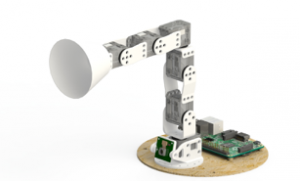
\includegraphics[width=178pt]{Ergo_Jr_abat_jour} 
    \caption{Le robot Ergo Jr avec un abat jour}
    \label{fig:ErgoJr}
\end{figure}

Dans ce rapport je vais d'abord présenter dans quel cadre j'ai pu travailler, puis je décrirais comment contrôler Ergo Jr ou un autre robot pour ensuite je vais détailler une autre méthode de contrôle et comment se déroule l'apprentissage.
Je terminerais ce rapport par montrer les résultats obtenus.

%%%%%%%%%%%%%%%%%%%
% % % CHAPTER % % %
%%%%%%%%%%%%%%%%%%%
% le cadre de travail, le descriptif de l’entreprise/le laboratoire
\chapter{Cadre de travail}

Ce stage s'est déroulé au \textbf{LORIA}, qui est le \textbf{L}aboratoire l\textbf{o}rrain de \textbf{R}echerche en \textbf{I}nformatique et ses \textbf{A}pplications.
C'est une \textbf{U}nité \textbf{M}ixte de \textbf{R}echerche (\textbf{UMR}) commune au CNRS, l'Université de Lorraine et Inria.
Depuis sa création en 1997, le Loria a pour mission la recherche fondamentale et appliquée en sciences informatiques.

Il est composé de 29 équipes structurées en 5 départements, dont 15 communes avec Inria, représentant un total de plus de 400 personnes.
Le Loria est un des plus grands laboratoires de la région lorraine.

\phantom{INVISIBLE LINE}

Ce stage se déroule au sein de l’équipe LARSEN (anciennement MaIA) qui a été créée au premier janvier 2015 et qui a pour responsable François Charpillet.
Cette équipe a pour objectif de faire évoluer des robots afin qu'ils atteignent des personnes en dehors des laboratoires de recherche et des industries.

Il faut donc des nouvelles méthodes afin que, à long terme, les robots soient autonomes, qu'ils développent des compétences relationnelles.
Ces compétences sont basées sur des interactions physiques et sociales.

\phantom{INVISIBLE LINE}

En raison de la situation sanitaire en France, la plus grande partie de ce stage s'est effectuée en télétravail. Les dernières semaines se sont passées en présentiel.

%%%%%%%%%%%%%%%%%%%
% % % CHAPTER % % %
%%%%%%%%%%%%%%%%%%%
% le sujet et son contexte 
\chapter{Présentation du stage}

Le robot Ergo Jr est un bras robotique. Il est composé d'une base, d'une suite de sections rigides et de moteurs, puis d'un effecteur (voir figure \ref{fig:SchemaErgoJr}). Il est contrôlé par une extension ajouté à un RaspberryPi qui est attaché à sa base.

\phantom{INVISIBLE LINE}

\begin{figure}[H]
    \centering
    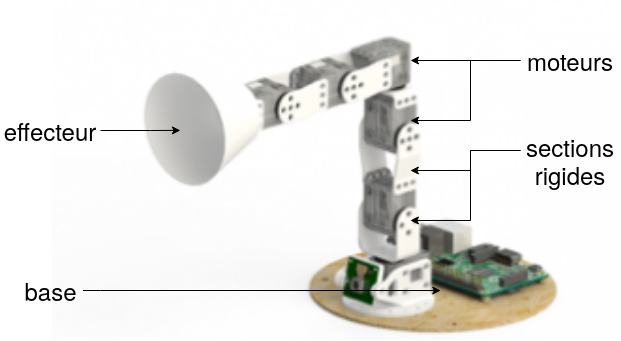
\includegraphics[height=140pt]{Ergo_Diagram} 
    \caption{Annotations sur le Ergo Jr}
    \label{fig:SchemaErgoJr}
\end{figure}

Le but de l'apprentissage n'est pas de contrôler la vitesse du robot mais seulement la position de son effecteur.
Je n'utiliserai donc pas la modélisation cinétique du robot mais seulement sa modélisation géométrique.

\phantom{INVISIBLE LINE}

Afin de déterminer la position de l'effecteur d'un bras robotique à partir d'une commande, donc d'une suite d'angle à appliquer à chacun de ses moteurs, il suffit de calculer le résultat des translations (les sections rigides) et des rotations (les moteurs).
Cela est simple lorsqu'il n'y a que des sections rigides et que le robot n'est pas soumis à beaucoup de contraintes, mais deviens très compliqué dans le cas contraire.

Passer d'une commande à la position de l'effecteur est le rôle de la modélisation géométrique directe.
Si la modélisation est difficile à construire, il est possible d'utiliser le monde réel comme modélisation: on donne la commande au robot et on observe la position de l'effecteur en résultat.
La réalité est le meilleure modèle physique que l'homme connaisse.

\phantom{INVISIBLE LINE}

Afin de déterminer quelle est la commande à executer afin d'atteindre avec l'effecteur une position donnée est le rôle de la modélisation géométrique inverse.
Il n'existe pas de modélisation géométrique universelle (directe ou inverse).
Elle est à calculer pour chaque robots.

De plus, lorsque le robot le permet comme Ergo Jr, il faut résoudre les problèmes de redondance: plusieurs commandes (plusieurs postures) permettent d'arriver à la même position de l'effecteur.

La construction du modèle géométrique inverse est souvent très compliquée, surtout si le robot est complexe.

\begin{figure}
    \centering
    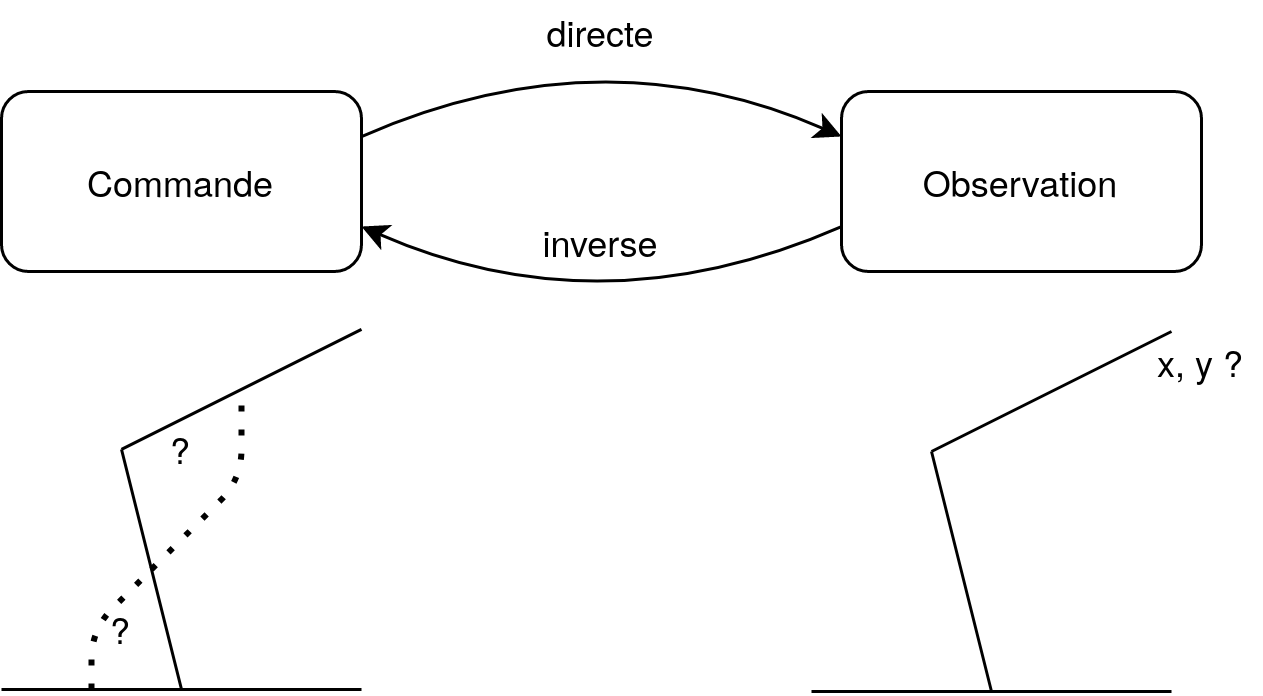
\includegraphics[height=140pt]{Modelisation_geometrique_diagram} 
    \caption{Représentation du rôle de la modélisation géométrique directe et inverse sur un bras robotique à une base et deux sections.}
    \label{fig:SchemaModelisation}
\end{figure}

\phantom{INVISIBLE LINE}

L'idée de ce stage est d'éviter de construire ces modèles, en s'inspirant de la nature.
Il n'y a pas de modèle géométrique qui dirige les mouvements d'un être vivant.
Un nouveau né ne va pas se déplacer autant et aussi précisément qu'un adulte, car celui-ci possède de l'expérience qu'il a acquis de son vivant.

C'est de ces processus dévelopementaux de systèmes biologiques que va s'inspirer un nouvel apprentissage.
Il va créer des robots qui ont une enfance et qui basent leurs décisions sur l'expérience acquise au cours du temps.
Le but est donc de créer un apprentissage qui permet d'acquérir de l'expérience et de la réutiliser afin de pouvoir controller le corps (ici un bras robotique).

%%%%%%%%%%%%%%%%%%%
% % % CHAPTER % % %
%%%%%%%%%%%%%%%%%%%
% le travail réalisé (résultats obtenus, démarche et méthode suivies, difficultés rencontrées, planning, ...)
\chapter{Travail réalisé}

Toute l'expérience acquise par le robot sera représentée par un catalogue liant des commandes et des observations.
Dans le cas du Poppy Ergo Jr, une commande est une liste d'angles données aux moteurs, et l'observation est la position dans l'espace de l'effecteur.

Tout le but de l'apprentissage est de créer, remplir et utiliser ce catalogue, qui est une manière de représenter toute l'expérience acquise dans la vie du robot.

\phantom{INVISIBLE LINE}

J'ai commencé mon stage par suivre un tutoriel \cite{TutoGoalBabling} de Fabien Benureau en python, qui explique les bases du Motor Babling et du Goal Babling sur un environnement en 2 dimensions.
Je l'ai ensuite adapté pour un environnement 3D.

J'ai d'abord crée un affichage 3D avec OpenGL et PyGame.
Puis j'ai appris à utiliser une bibliothèque Poppy Ergo Jr, basé sur PyPot \cite{PyPot} et Ikpy \cite{IKPy}.
Je me suis ensuite renseigné sur les différents algorithmes de Nearest Neighbor disponibles en python pour l'intégrer au projet.
Enfin j'ai ajouté une méthode Frontier \cite{Frontier} pour finaliser l'apprentissage.

\pagebreak
%%%%%%%%%% SECTION %%%%%%%%%%
\section{Utilisation du catalogue}

Une fois un catalogue créé et rempli, nous pouvons l'utiliser afin de controller le robot.
Lorsque l'utilisateur (ou le robot) décide d'atteindre une certaine position avec l'effecteur, il suffit de recherche l'observation dans le catalogue la plus proche du point demandé et d'exécuter la commande associée.

Le robot reçoit  alors une liste d'angle pour déterminer sa posture et son effecteur arrivera donc à l'observation du catalogue, qui est proche du point demandé.

\phantom{INVISIBLE LINE}

Le problème de cette solution est que le robot s'approche du point demandé sans l'atteindre.
Le catalogue contient un nombre fini de points, ce qui ne rempli pas continuellement l'espace.

Une deuxième solution qui permet d'utiliser le catalogue, tout en offrant des résultats dans un espace continu, est de rechercher plusieurs observations les plus proches de la position demandée.

Il faut ensuite faire une moyenne sur les commandes associées, pondérée par la distance entre l'observation et le but.
Le robot peut ainsi atteindre un espace continu à partir d'un catalogue de taille finie.

\phantom{INVISIBLE LINE}

Pour utiliser le catalogue rapidement, il faut rapidement trouver l'observation la plus proche du but.
C'est exactement ce que fait l'algorithme de Nearest Neighbor (plus proche voisin).
Pour pouvoir utiliser un Nearest Neighbor dans ce projet, il faut qu'il puisse réspecter trois contraintes:
\begin{itemize}
    \item Une recherche rapide d'un plus proche voisin
    \item La possibilité de rechercher un groupe de plus proches voisins
    \item Facilité à ajouter des données en parallèle d'utilisation
\end{itemize}
Cette dernière contrainte est importante car lors de l'apprentissage (le remplissage du catalogue), ce Nearest Neighbor sera utilisé.

\pagebreak
%%%%%%%%%% SECTION %%%%%%%%%%
\section{Remplir le catalogue}

Je vais ici présenter les trois méthodes utilisées pour remplir le catalogue.
Toutes sont basées sur le babillage des mouvements d'un nouveau né.

La premère méthode est le Motor Babling, en français babillage moteur.
Elle permet d'explorer l'espace moteur du robot et est simple à mettre en place.

\phantom{INVISIBLE LINE}

Ensuite nous verrons la catégorie Goal Babling \cite{GoalBabling}, pour un babillage par but.
Dans cette catégorie, l'apprentissage génère des buts.
C'est la décision prise, la sélection d'un but, qui permet de diriger l'apprentissage et d'explorer l'espace de travail plutôt que l'espace moteur.

Il existe plusieurs algorithmes permettant de générer des buts.
L'un d'eux est le Agnostic Goal Generator (génération agnostique de but).
Il est appellé agnostique car les buts sont générés sans avoir d'informations sur le robot, qui se comporte comme une boîte noire.
Des commandes lui sont envoyés et il renvoie une position.

Ensuite je présenterais une catégorie de générateur de but, les Goals on Grid.
Ces algorithmes se basent sur une discrétisation de l'espace pour générer des buts, d'où la "grille de but".
Ici la difficultée sera de choisir une certaine cellule dans la grille, ce qui peut être fait avec l'algorithme Frontier.

\begin{algorithm}[h]
    \DontPrintSemicolon
    \LinesNumbered
    $cat \leftarrow Catalogue$\;
    \For { $1 \le i \le N $} {
        $c \leftarrow newCommand(cat)$ \;
        $o \leftarrow Robot.execute(c)$\;
        $cat.add(c, o)$ \;
    }
    \caption{\label{alg:Fill} Fill}
\end{algorithm}

%%% SUB - SECTION %%%
\subsection{Motor Babling}

Une première approche pour que le robot acquière de l'expérience est une exploration de ses espaces moteurs et sensoriels.
Ceci est comparable au comportement d'un nouveau né qui ne contrôle pas ses mouvements.

\phantom{INVISIBLE LINE}

Le robot va d'abord prendre une posture aléatoire, donc choisir pour chaque moteurs et dans leurs limites un angle aléatoire selon une distribution uniforme.
Ensuite il va observer en résultat la position de son effecteur dans le monde.

Ceci est un babillage moteur (en anglais Motor Babling).
Nous construisons ainsi un catalogue, contenant toutes les postures essayées et les observations associées, qui constitue la mémoire et l'expérience du robot.

\begin{algorithm}[h]
    \DontPrintSemicolon
    \LinesNumbered
    $command \leftarrow \emptyset$ \;
    \ForEach{$m \in Robot.Motors$}{
        $c \leftarrow random(m.min, \hspace{5pt} m.max)$ \;
        $command.append( c )$\;
    }
    \Return{command}
    \caption{\label{alg:MotorBabling} MotorBabling}
\end{algorithm}

%%% SUB - SECTION %%%
\subsection{Goal Babling}

L'exploration de l'espace des moteurs du robot ne permet pas toujours d'explorer efficacement l'espace de travail du robot.
La distribution des observations du catalogue dans l'espace de travail ne sera pas uniforme.

Si certaines zones sont facilement atteignables et qu'il existe un grand nombre de redondances pour atteindre les points de cette zone, une exploration de l'espace moteur va automatiquement se concentrer sur cette zone.

\phantom{INVISIBLE LINE}

Cepentant, il est possible de diriger l'apprentissage en choisisant des but à atteindre.
C'est donc un babillage par but, ou Goal Babling en anglais.

Cette méthode est une manière de représenter la motivation intresèque: la décision qui est de choisir le but est prise par le robot et non par un utilisateur extérieur, afin de maximiser l'expérience acquise \cite{Intrinsic_motivation}.

\phantom{INVISIBLE LINE}

La sélection de but permet de diriger l'exploration pour sortir des zones facilement atteignables, afin d'atteindre tout l'espace de travail.
Cependant, si tous les buts générés sont mal positionnés, l'utilisation du catalogue donnera des résultats peu précis.

Il existe plusieurs façons de générer un but.
Je vais décrire deux méthodes: la génération de but agnostique, et la génération de but sur une grille à l'aide de l'algorithme Frontier.

\begin{algorithm}[h]
    \DontPrintSemicolon
    \LinesNumbered
    $cat \leftarrow Catalogue$\;
    $goal \leftarrow GenerateGoal(cat)$ \;
    $c, o \leftarrow cat.nearest(goal)$ \;
    $command \leftarrow c.perturb()$ \;
    \Return{command}
    \caption{\label{alg:GoalBabling} GoalBabling}
\end{algorithm}

% SUB - SUB %
\subsubsection{Agnostic Goal Generation}

Afin d'explorer uniformément l'espace de travail, il est possible de créer des buts uniformément sur cet espace.
Cepandant les buts sont générés sans aucune connaissance au préalable sur le robot, donc aucune connaissance sur son espace de travail.
C'est pour cela que ce générateur de but est agnostique.

\phantom{INVISIBLE LINE}

Afin de pouvoir approximer l'espace de travail du robot, les positions extrêmes (les minimums et maximums sur chacun des axes) sont enregistrées.
En résultat nous avons une zone que le robot peut potentiellement atteindre.
Le prochain but sera généré dans cette zone, dont la taille sera mutlipliée par un facteur, qui déterminera ainsi le taux d'exploration.

\phantom{INVISIBLE LINE}

Cependant, cette méthode ne fait qu'approximer l'espace de travail qui est rarement un simple cube (ou pavé droit).

\begin{algorithm}[h]
    \DontPrintSemicolon
    \LinesNumbered
    $Cat \leftarrow Catalogue$ \;
    $Ext \leftarrow CoefExtension$ \;
    $goal \leftarrow \emptyset$ \;
    \ForEach{$\{x, y, z\}$ }{
        $min \leftarrow Cat.min() \times Ext$ \;
        $max \leftarrow Cat.max() \times Ext$ \;
        $val \leftarrow random(min, \hspace{5pt} max)$ \;
        $goal.append(val)$ \;
    }
    \Return{goal}
    \caption{\label{alg:Agnostic} Agnostic}
\end{algorithm}

\pagebreak

% SUB - SUB %
\subsubsection{Goals on Grid et Frontier}

Afin d'approcher encore plus l'espace de travail du robot sans avoir de connaissance sur celui-ci, il est possible de partitionner l'espace en une grille.
Lors de l'apprentissage, toutes les cellules atteintes par les observations du catalogue sont enregistrées, ce qui nous donne une estimation sur l'espace atteint.
On obtient ainsi, avec une certaine résolution, une représentation de l'espace atteint pendant l'apprentissage.

\phantom{INVISIBLE LINE}

L'algorithme de Goals on Grid est une adaptation en 3 dimensions de celui présenté dans la thèse de Fabien C. Y. Benureau \cite{TheseBenureau}.
L'idée de partitionner l'espace pour le Goal Babling a été utilisé dans le contexte de l'algorithme SAGG-RIAC \cite{Intrinsic_motivation}.

\phantom{INVISIBLE LINE}

Une fois cette représentation obtenue, s'il faut augmenter la précision du catalogue (exploitation), le prochain but sera généré dans une cellule déjà atteinte.
Si, au contraire, il faut augmenter la couverture (exploration), le prochain but sera généré dans une cellule non atteinte.

\begin{algorithm}[h]
    \DontPrintSemicolon
    \LinesNumbered
    $Cat \leftarrow Catalogue$ \;
    $p \leftarrow ExplorationProbability$ \;
    $visited \leftarrow VisitedCells$ \;
    $r \leftarrow random()$ \;
    \If{$r \le p$}{
        $c \leftarrow selectNonVisitedCell(visited)$ \;
        $visited.append(c)$ \;
    }
    \Else{
        $c \leftarrow random(visited)$ \;
    }
    $goal \leftarrow GenerateGoalInCell(c)$ \;
    \Return{goal}
    \caption{\label{alg:GoalsOnGrid} GoalsOnGrid}
\end{algorithm}

\textbf{Frontier Goal Generation}

\phantom{INVISIBLE LINE}

L'algorithme frontier permet de selectionner une cellule non atteinte mais potentiellement atteignable. L'idée principale de cet algorithme, décrit dans la thèse de F. Benureau \cite{TheseBenureau} peut être reconnue dans l'algorithme Goal Directionnal Sampling de Rolf \cite{Frontier}.

Premièrement, une observation dans le catalogue est selectionnée aléatoirement.
Ensuite, une direction est aussi générée aléatoirement en selectionnant uniformément un point sur la surface d'une sphère.

\phantom{INVISIBLE LINE}

L'algorithme parcours ensuite la grille à partir de l'observation, en suivant la direction jusqu'à rencontrer une cellule qui n'est pas encore atteinte.
Cette cellule est donc à la frontière de la zone atteinte par le robot.
L'algorithme Frontier permet donc d'explorer un espace plus proche de l'espace de travail que l'algorithme Agnostic.

\begin{algorithm}[h]
    \DontPrintSemicolon
    \LinesNumbered
    $visited \leftarrow VisitedCells$ \;
    $Cat \leftarrow Catalogue$ \;
    $_, o \leftarrow random(Cat)$ \;
    $cell \leftarrow o \div Cell.size$ \;
    $dir \leftarrow generateRandomDir()$ \;
    \While{$cell \in visited$}{
        $cell \leftarrow nextCell(cell, \hspace{5pt} dir)$ \;
    }
    \Return{cell}
    \caption{\label{alg:Frontier} Frontier}
\end{algorithm}


%%%%%%%%%%%%%%%%%%%
% % % CHAPTER % % %
%%%%%%%%%%%%%%%%%%%
\chapter{Observations}

%%%%%%%%%% SECTION %%%%%%%%%%
\section{Mesures}

Afin de pouvoir comparer différents algorithmes, je vais mesurer la couverture du catalogue ainsi que la précision du résultat.

\phantom{INVISIBLE LINE}

\textbf{Couverture}

\phantom{INVISIBLE LINE}

La couverture sera mesurée à partir de ces deux valeurs:

\begin{itemize}
    \item[$\bullet$] Le volume, qui est le volume de l'enveloppe convexe des points du catalogue et le volume d'une zone théoriquement atteignable par le robot.
    Cela permet de mesurer la taille de l'espace couvert par l'algorithme et déterminer un taux d'exploration.
    \item[$\bullet$] Le remplissage, qui est le le nombre de cellules de la discrétisation de l'espace qui contiennent au moins une observation du catalogue.
    Cela permet de mesurer le taux de remplissage de l'espace couvert.
\end{itemize}
Ces valeurs sont normalisées avec un volume (ou un nombre de cellules) théoriquement atteignable.
J'ai choisi pour ce volume une sphère dont le rayon est la taille du bras robotique.

\phantom{INVISIBLE LINE}

\textbf{Precision}

\phantom{INVISIBLE LINE}

La précision sera déduite à partir de l'erreur, qui est la distance entre un but donné et l'observation générée par le résultat du modèle inverse.
Les mêmes buts seront utilisés pour comparer tous les algorithmes.
Deux listes de but ont été retenues:

\begin{itemize}
    \item[$\bullet$] La première liste contient des buts générés aléatoirement selon une distribution uniforme dans un espace théoriquement atteignable par le robot.
    L'espace selectionné est 3/4 d'une demi-sphère.
    Il est inutile de demander au robot d'atteindre une zone sous sa base, il ne peut pas traverser une table, cela enlève une demi-sphère.
    Nous ne demandons pas au robot d'essayer d'atteindre une zone "derrière lui", ce qui exclue 1/4 de la zone restante.
    Voir figure \ref{fig:goal_list} pour une représentation vue de face et du dessus.
    
    \begin{figure}
        \centering
        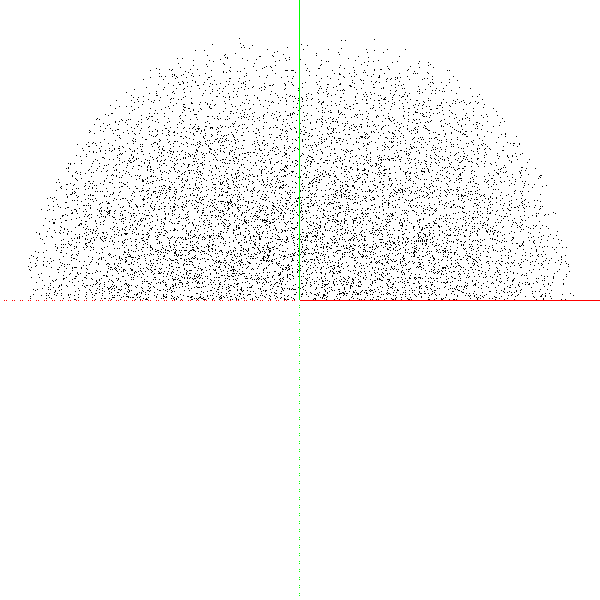
\includegraphics[width=178pt]{goal_list_front} 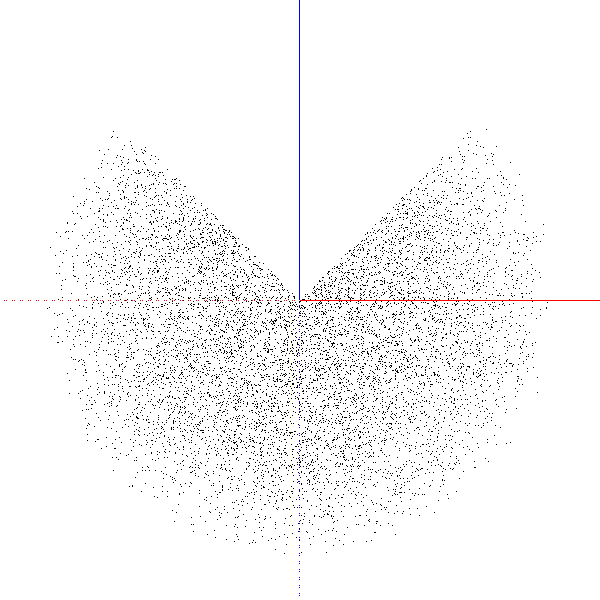
\includegraphics[width=178pt]{goal_list_top}
        \caption{Représentation de la première liste des buts}
        \label{fig:goal_list}
    \end{figure}
    
    \item[$\bullet$] La deuxième liste contient les observations faites après utilisation d'un modèle inverse existant dans une bibliothèque, appellée Ikpy.
    Cette liste ne contient que des observations, donc des points qui sont réellement atteignables.
    Avec ce modèle inverse, il est possible de comparer l'efficacité d'un modèle inverse existant, ici Ikpy \cite{IKPy}, avec le modèle inverse généré par les algorithmes.
\end{itemize}

\pagebreak

%%%%%%%%%% SECTION %%%%%%%%%%
\section{Paramètres}

Il existe plusieurs paramètres aux différents algorithmes utilisés.
Afin de pouvoir les comparer, il faut d'abord trouver les paramètres les plus optimisés pour chacune des instances.

\phantom{INVISIBLE LINE}

Un paramètre commun à tous ces apprentissage est donc la taille du catalogue, ou plus précisément le nombre d'entrées dans le catalogue.

Deux valeurs ont étées testées pour ce paramètre.
La première valeur est 1 000 entrées dans le catalogue pour représenter une borne inférieure.
La deuxième est 100 000 entrées dans le catalogue, qui est une borne supérieur par rapport au temps de calcul et l'espace disque utilisé.

%%% SUB - SECTION %%%
\subsection{Motor Babling}

\`A chaque étape du Motor Babling, une posture est choisie en donnant un angle aléatoire à chacun des moteurs généré uniformément sur leur portée.
C'est une exploration de tout l'espace moteur du robot, donc tout point atteignable par ce robot possède donc une probabilité non nulle d'être dans le catalogue.
J'en déduis que la couverture du Motor Babling augmente avec la taille de son catalogue.

Sur la figure \ref{fig:MB_couv_remp}, il y as une différence très significative (****) entre les données, et plus d'étapes montrent une meilleure couverture et un meilleure remplissage

\begin{figure}[h]
    \centering
    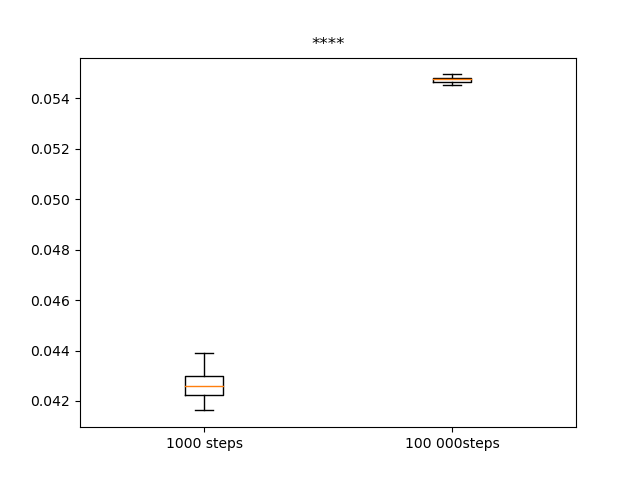
\includegraphics[width=178pt]{1mb_1k-100kstep_couver.png} 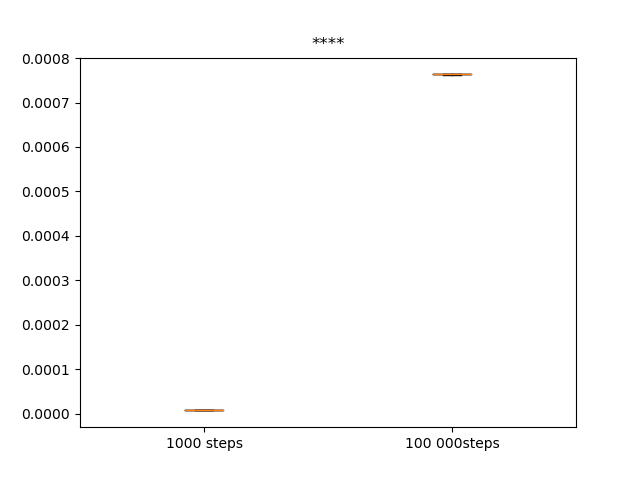
\includegraphics[width=178pt]{1mb_1k-100kstep_rempli.png}
    \caption{Couverture (gauche) et Remplissage (droite) des catalogues pour 1000 et 100 000 entrées sur du Motor Babling.}
    \label{fig:MB_couv_remp}
\end{figure}

Avec plus d'entrée dans le catalogue, il y aura plus d'observations proche d'un but. L'interpolation utilisera donc des points plus proches, ce qui augmente la précision du résultat de l'algorithme.

Sur la figue \ref{fig:MB_dis_moy}, il y aussi une différence très significative. Cela confirme que plus d'entrées dans la base donnent une distance moyenne entre résultat et but plus petite donc une meilleure précision.

\begin{figure}[h]
    \centering
    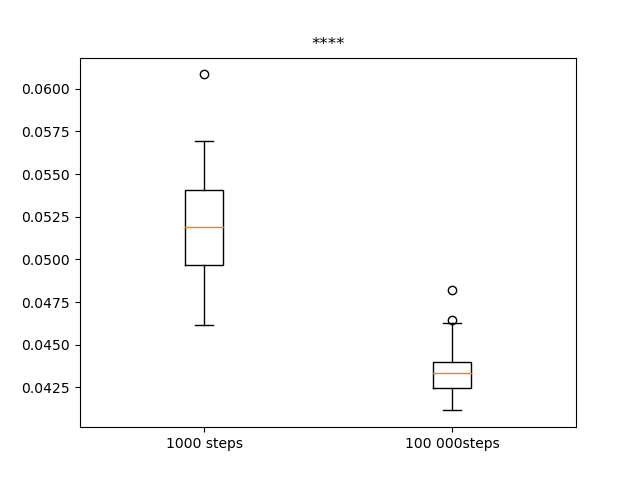
\includegraphics[width=178pt]{1mb_1k-100kstep_moy_ik.png} 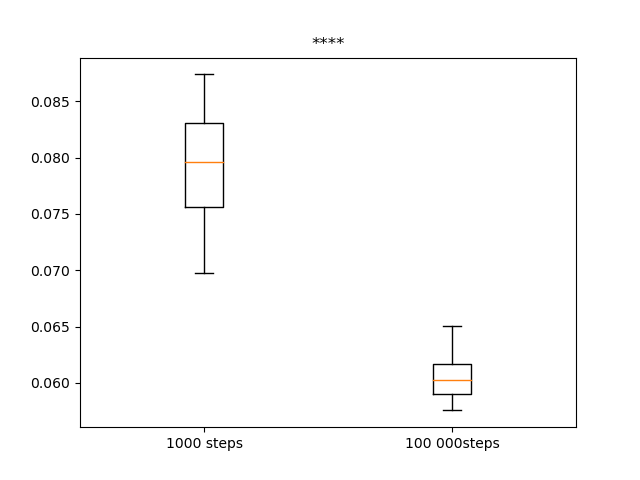
\includegraphics[width=178pt]{1mb_1k-100kstep_moy_gl.png}
    \caption{Distance moyenne des observations à la liste des but (gauche), et à la liste Ikpy (droite) pour 1000 et 100 000 entrées.}
    \label{fig:MB_dis_moy}
\end{figure}

%%% SUB - SECTION %%%
\subsection{Goal Babling}

Quelque soit l'algorithme de génération du but, pour initier le Goal Babling il faut exécuter un certain nombre d'étapes de Motor Babling.
C'est donc un paramètre à prendre en compte.

Comme il faut commencer par un certain nombre d'étapes de Motor Babling, la borne inférieure testée pour ce paramètre est une proportion de 0.01 étapes sur le nombre total d'entrées du catalogue.
Si la proportion est de 1, cela revient à faire simplement du Motor Babling. Une proportion trop grande pollue trop le catalogue avec du Motor Babling, ce qui va cacher les résultats de l'algorithme utilisé pour le Goal Babling.
La deuxième valeur testée pour ce paramètre est une proportion de 0.2 sur le nombre total d'entrée du catalogue.

La figure \ref{fig:effet_mb_prop}, les différences entre les couvertures et les précisions sont très significatives.
La meilleure couverture avec 0.01 ou 0.2 en proportion de motor babling change peu.
Ce n'est que dans certains cas qu'une mauvaise initialisation perturbe le Goal Babling.
La même observation peut être faite sur la précision.

\begin{figure}[h]
    \centering
    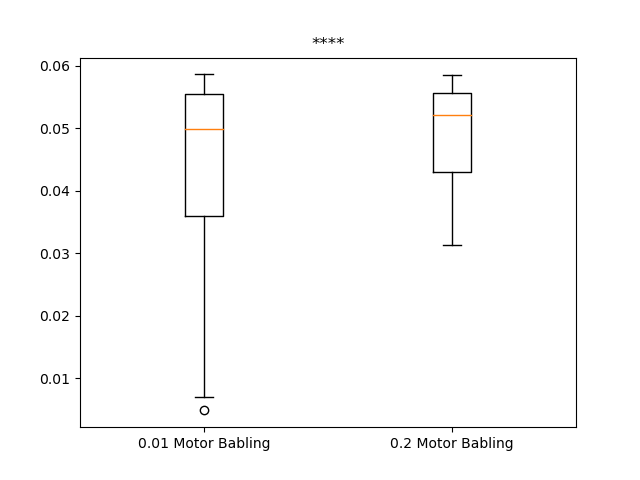
\includegraphics[width=160pt]{0.2-.01mb_couver.png} 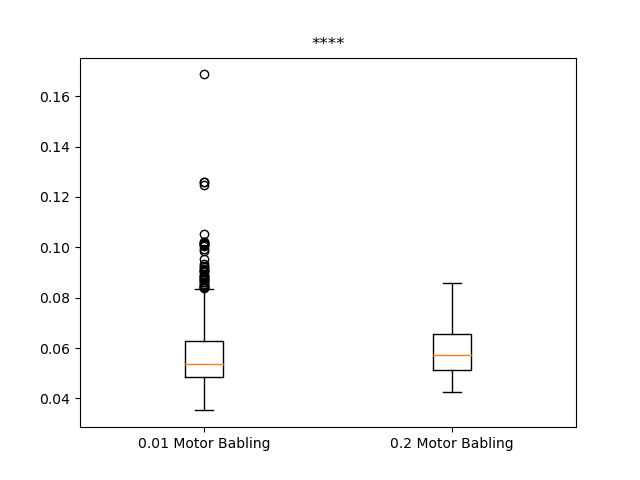
\includegraphics[width=160pt]{0.2-.01mb_moy_gl.png}
    \caption{Couverture (gauche) et Précision (droite) pour deux proportions de Motor Babling.}
    \label{fig:effet_mb_prop}
\end{figure}

\phantom{INVISIBLE LINE}

Lorsqu'un but est choisi, une nouvelle entrée dans le catalogue est crée à partir d'une perturbation de donnée existante.
Cette perturbation est un autre paramètre à prendre en compte pour du Goal Babling.
Avec une perturbation plus elevée, la posture générée sera normalement plus loin de la posture selectionnée.
La couverture d'un algorithme augmente donc avec la perturbation.

Une observation sur une posture grandement perturbée a plus de chance d'être distante du but demandé.
Cette perturbation peut donc détériorer la précision de l'algorithme.
Les valeurs utilisées pour ce paramètre sont une proportion de 0.05 de la portée du moteur, ainsi qu'une proportion de 0.2 de la portée du moteur.

Sur la figure \ref{fig:effet_pp}, Les résultats sont similaires à l'impacte de la proportion de Motor Babling.
Une bonne perturbation est necessaire pour explorer correctement l'espace.

\begin{figure}[H]
    \centering
    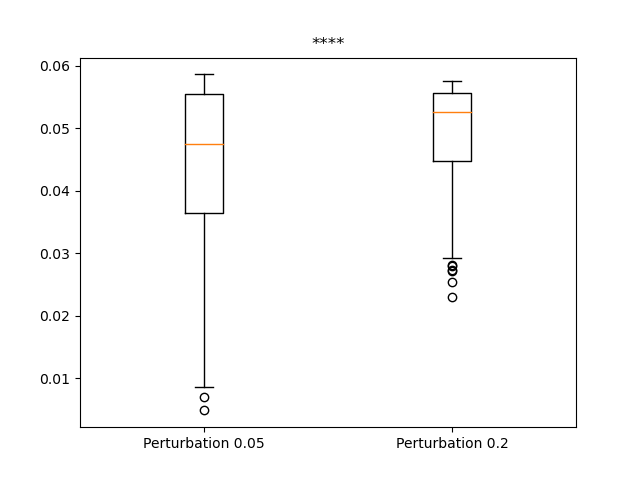
\includegraphics[width=160pt]{0.05-.2pp_couver.png} 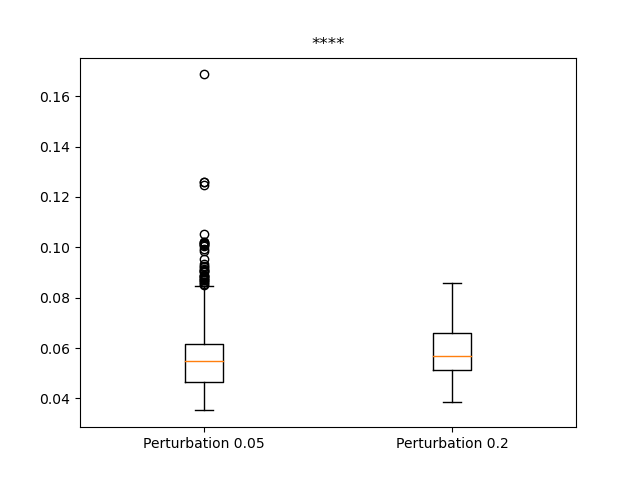
\includegraphics[width=160pt]{0.05-.2pp_moy_gl.png}
    \caption{Couverture (gauche) et Précision (droite) pour deux perturbations de posture.}
    \label{fig:effet_pp}
\end{figure}

\pagebreak

%%% SUB - SECTION %%%
\subsection{Agnostric Goal Generation}

La génération de but agnostique utilise une zone qui est calculée à partir de la zone couverte par les observations du catalogue.
Afin d'ajouter un taux d'exploration à l'algorithme, la zone de génération des buts sera une extension de la zone couverte par le catalogue.

Plus le coefficient d'extention de cette zone est grand, plus la zone de génération de but est grande.
Or le nombre d'entrée du catalogue ne change pas, ils sont donc plus dispersés.
Ce coefficient impacte donc positivement la couverture mais négativement la précision.

Deux valeurs sont utilisées pour ce paramètre.
La première est de 0.7, une borne inférieure qui permet d'illustrer si un autre paramètre impacte plus l'exploration que celui-ci.
La deuxième est 1.4, valeur supposée non extrême: une valeur trop grande donne une génération de but impossible à atteindre.

Sur la figure \ref{fig:effet_exp}, un coefficient d'extension plus grand donne une meilleure couverture avec une différence très significative sur les données (****).
La précision est un peu moins impactée mais est meilleure avec une extension plus faible.

\begin{figure}[h]
    \centering
    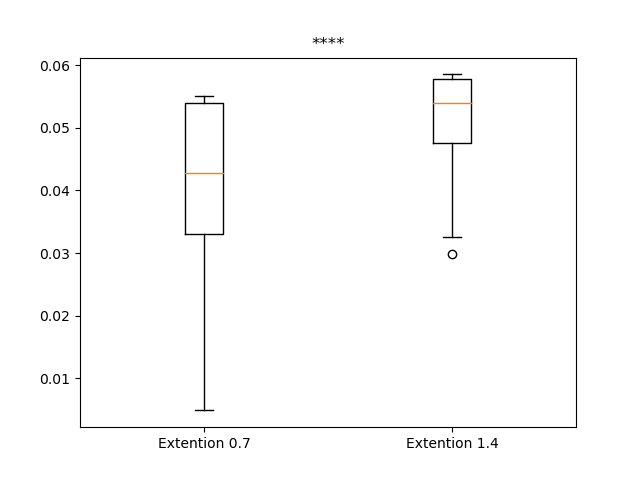
\includegraphics[width=178pt]{Agn_.7-1.4exp_couver.png} 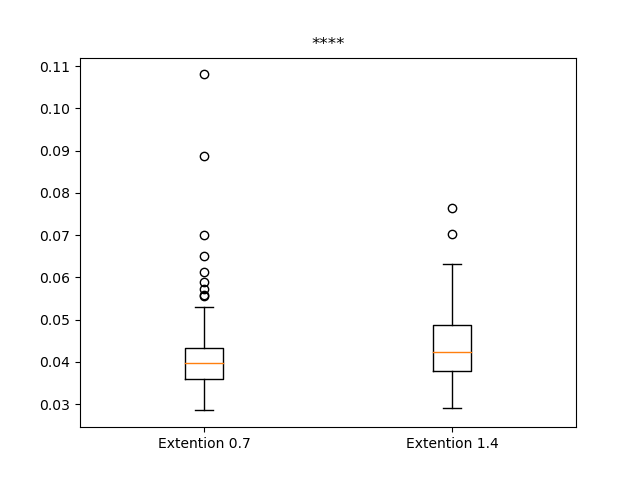
\includegraphics[width=178pt]{Agn_.7-1.4exp_moy_ik.png}
    \caption{Couverture (gauche) et Précision (droite) pour deux coefficients d'extension.}
    \label{fig:effet_exp}
\end{figure}

\pagebreak

%%% SUB - SECTION %%%
\subsection{Frontier Goal Generation}

Lors de l'utilisation du Frontier Goal Generator, ou plus largement du Goals on Grid, il existe un coefficient d'exploration p.
Avec une probabilité p l'algorithme va choisir d'explorer l'espace, et avec une probabilité 1-p, l'algorithme choisi d'exploiter le catalogue.
Trois valeurs de p ont été testées.
Les bornes 0.01 et 0.9, ainsi qu'une valeur intermédiaire 0.5.

Cependant, comme le montre la figure \ref{fig:effet_pexp}, ce paramètre n'impacte pas les résultats.
Il n'y a pas (ou très peu <*>) de différences entre les distributions de couverture et de précision (\textbf{N}o \textbf{D}ifference).

\begin{figure}[h]
    \centering
    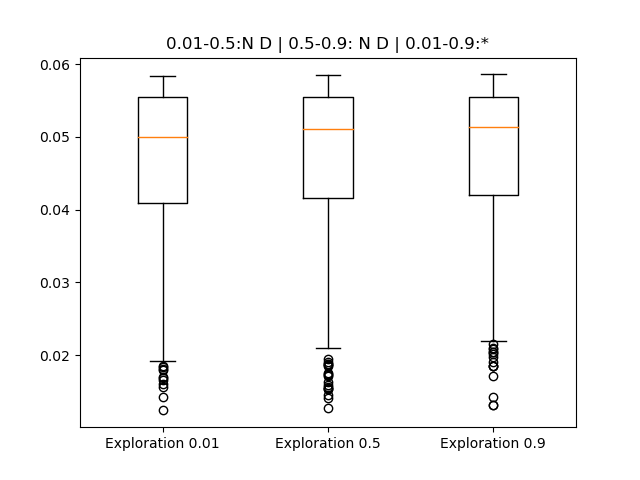
\includegraphics[width=178pt]{Fro_.01-.5-.9pexp_couver.png} 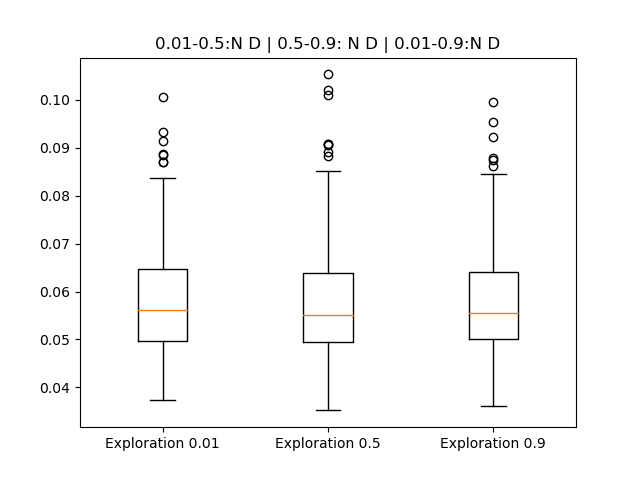
\includegraphics[width=178pt]{Fro_.01-.5-.9pexp_moy_gl.png}
    \caption{Couverture (gauche) et Précision (droite) pour deux probabilités d'exploration.}
    \label{fig:effet_pexp}
\end{figure}

Il est aussi possible de changer la taille d'une cellule pour l'utilisation de Goals on Grid.
Une taille de cellule plus petite représentera plus précisemment la zone atteinte par le catalogue, mais rendra l'exploration de l'espace plus lente.
Avec une taille de cellule trop grande, l'algorithme se résume à une génération de but dans une zone spécifié: la cellule englobant le robot.
J'ai choisi de fixer la taille de l'espace, et je détermine la taille d'une cellule à partir d'un certain nombre de division de cet espace.
Deux valeurs pour ce paramètre ont été testée: 10 divisions (pour des cellules de 10cm\up3), et 1 000 divisions (pour des cellules de 1mm\up3).

La résolution de la discrétisation possède par contre un effect plus significatif sur les résultats que la probabilité d'exploration, comme le montre la figure \ref{fig:effet_res}.
Une résolution plus grande, et donc des cellules plus petites, rend plus difficile l'exploration.
La précision est aussi impactée négativement avec l'augmentation de la résolution.

\begin{figure}[h]
    \centering
    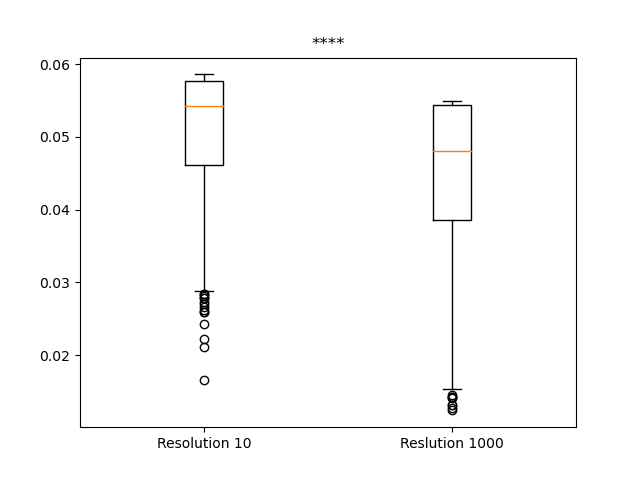
\includegraphics[width=178pt]{Fro_10-1kres_couver.png} 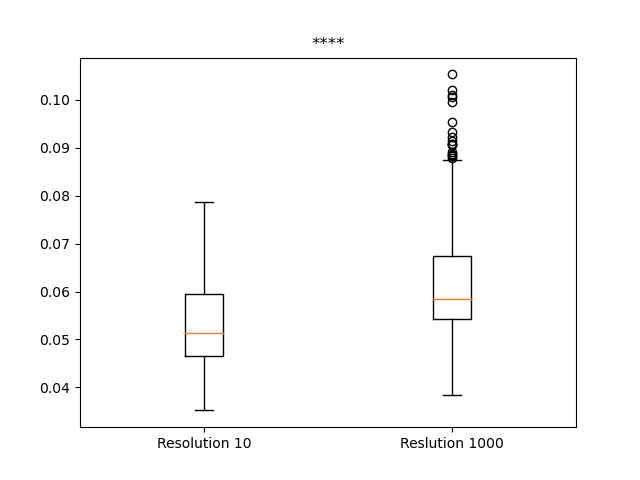
\includegraphics[width=178pt]{Fro_10-1kres_moy_gl.png}
    \caption{Couverture (gauche) et Précision (droite) pour deux résolution de discrétisation.}
    \label{fig:effet_res}
\end{figure}

%%%%%%%%%%%%%%%%%%%
% % % SECTION % % %
%%%%%%%%%%%%%%%%%%%
% les conclusions
\chapter{Conclusion}

% Rappel du sujet,
L'objectif de ce stage est d'appliquer la méthode du Goal Babling \cite{GoalBabling} sur le robot Poppy Ergo Jr \cite{PoppyErgoJr}.
Pour ce projet j'ai utilisé Python et certaines bibliothèques comme Ikpy \cite{IKPy}, RTree \cite{RTree} et OpenGL.

J'ai débuté par une introduction au Goal Babling présenté par Fabien Benureau \cite{TutoGoalBabling}.
Puis j'ai adapté cette solution pour un espace de dimension 3, en ajoutant des méthodes pour l'affichage.
J'ai effectué des recherches sur une bibliothèque de Nearest Neighbor la plus adaptée à cet apprentissage, pour enfin utiliser un RTree \cite{RTree}.
J'ai ensuite appliqué une méthode présentée dans la thèse de Mr Benureau \cite{TheseBenureau}, en adaptant le principe au programme.
Enfin, j'ai appris l'utilisation de certains outils afin d'effectuer efficacement plusieurs apprentissages pour obtenir les résultats.

Les résultats obtenus ne sont pas utilisables sur le robot réel, car les contraintes physiques ont été ignorées pendant l'apprentissage.
Certaines postures sont impossibles à réaliser par exemple quand le bras robotique se traverse pour atteindre sa posture.
La précision est aussi assez faible, les résultats donnés étant distants en moyenne à 0.04 unités du but demandé, qui correspond normalement à 4 cm.

En ajoutant des contraintes et en donnant plus de temps à l'apprentissage, un robot pourrait être contrôlé avec une grande précision et en mettant en oeuvre toutes ses capacités.
Ajouter aussi une orientation à l'apprentissage est possible, du moment que le calcul de distance et le Nearest Neighbor soientt adaptés.

Avec ce sujet j'ai pu explorer une autre façon de contrôler un robot que celles qui m'ont été présentées lors de mon année scolaire.
Cette méthode d'apprentissage est aussi nouvelle pour moi.

Même si les conditions de travail étaient exceptionnelle, ce stage m'a permis de conclure mes années d'études et m'a donné un apperçu du travail de chercheur.

%%%%%%%%%%%%%%%%
% BIBLIOGRAPHY %
%%%%%%%%%%%%%%%%
\bibliographystyle{unsrt}
\bibliography{sample}

\end{document}
